
\section{Mars Gravity Coordinate Frame} \label{sec:Marsg} 
The inertial system for Mars is that defined by the IAU for solar system bodies, namely the ICRF centered on Mars \ref{sec:gen}.
The fixed frame for mars should be the one associated with its fitted gravitational field, see \ref{sec:Marsg}. As of this writing, the Mars gravity model will be MRO110B \cite{2011Icar}.
The document \cite{2006Icar} defines the rotation relation between inertial and fixed coordinates by the angles:
\begin{itemize}
\item The angle N is from the vernal equinox to the node of the Mars mean orbit plane.
\item J is the inclination of Mars mean orbit to the ICRF x-y plane.
\item $\psi$ is the angle from the mean orbit relative to the ICRF x-y plane.
\item I is the inclination of the Mars true equator of date relative to Mars mean orbit.
\item $\phi$ is the spin angle from the node of the Mars true equator of date to prime meridian of Mars, see figure \ref{fig:7a}. 
\end{itemize}

The inertial to Mars fixed transformation is described in JEOD Environment - Mars RNP document.

\textbf{Coordinate Frame: } Rotating 

\begin{itemize}
\item X-axis: Points in the direction of the prime meridian of Mars.
\item Y-axis: Completes a standard, right-handed coordinate frame.
\item Z-axis: Defined as the pole vector of the Mars Mean Equator.
\end{itemize}

\begin{figure}[htp]
\centering
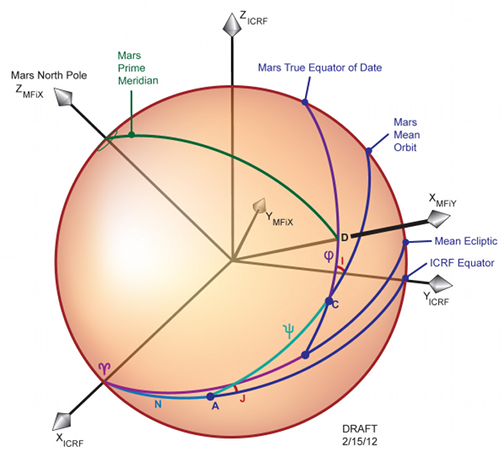
\includegraphics [width=7in]{figs/fig7a.png}
\caption{Mars Gravitational Fixed System}
\label{fig:7a}
\end{figure}

\subsection{Example MARS RNP}
See the JEOD \hypermodelref{RNP} for examples.